% vim: set fenc=utf-8 ft=latex encoding=utf-8
% -*- mode: latex; coding: UTF-8; -*-
%!TEX root = knowledge-curation.tex
\section{Theory and Discussion}
\label{cha:theory}

    In this section we present a theory that encapsulates the observations and insights found during the analysis of the data, including, the comparison of the way knowledge is shared on both channels, and the recommendations of the use of Q\&A media channels.
    We also discuss them with respect to the related literature.

%Categorization of the way resources are used on Q\&A media channels.
\subsection{How the knowledge is shared on channels}

    Based on the categorization performed, both channels provide roughly the same knowledge support for questions and answers.
    However, there are some differences between both channels which are summarized in Table~\ref{table:constrat}.
    These observations are tendencies, and they are not behaviours unique of each channel.

    \begin{table}[!htb]
      \centering
      \caption{Comparison of the way knowledge is shared on Stack Overflow and the R-help mailing list.}
      \label{table:constrat}
      \begin{small}
          \setlength{\tabcolsep}{5pt}
          \begin{tabular}{@{}lll@{}}
            \toprule
            \textbf{}      & \textbf{Stack Overflow} & \textbf{R-help}\\
            \midrule
            Knowledge construction & Crowd             & Participatory \\
            Topic restriction      & Topic restriction & No topic restriction \\
            Knowledge              & Curated knowledge & Knowledge development\\
            \bottomrule
          \end{tabular}
      \end{small}
    \end{table}

    Stack Overflow is more suitable for questions with a clear answer, and the R-help mailing list is more suitable to discuss topics that are in and out of the software development domain.
    The study by Squire~\cite{Squire2015a} presents a similar difference between Stack Overflow and a mailing list of multiple projects through a different approach.
    
    The main benefit of using crowd knowledge construction is the existence of a pool of solutions, which combined with curation mechanisms, produces multiple ways to solve the same problem (diversity of solutions) in a clear solution that can be reused.

\subsubsection{Knowledge construction}

    Stack Overflow's gamification system encourages participation by giving points to those who participate~\cite{Singer2013}.
    Even when the diversity of answers provided in Stack Overflow is high, users tend to not contribute (edit or comment) in such answers; instead, some users provide their own answers.
    For instance, in the Stack Overflow thread \textit{\href{http://goo.gl/Mb4Pbk}{``Resources for learning SAS if you already familiar with R''}}, three of the six answerers referenced the same books.
    The gamification mechanism gives reputation to those who answer the questions, even when each extra answer might not add any new insight about how to solve a specific problem.
    Stack Overflow curation mechanism provides information about the popularity of answers, but not why, or how it is better than others answers.

    In contrast, the R-help mailing list tends to be more collaborative on how users construct knowledge, and discuss proposed answers.
    Participants of the R-help mailing list tend to provide more background to the answers as well as to explain answers of other participants.
    For example, the question \textit{``Arrange elements on a matrix according to rowSums + short `apply' Q''} was posted on both \href{http://goo.gl/a8AES8}{Stack Overflow} and \href{http://goo.gl/PGflT5}{R-help} mailing list.
    Both communities answered the question using a different knowledge construction approach.
    On Stack Overflow, each participant provided their own solution without any evidence of collaboration between them.
    Whereas users on the R-help mailing list complemented each other answers by providing extra information.

    The Stack Overflow's knowledge construction is not limited to crowd knowledge construction, it also presents collaborative ways to construct knowledge.
    However, the crowd one seems more prevalent.
    On the R-help mailing list happens the same as on Stack Overflow, but the other way around.

    Tausczik \textit{et al}.~\cite{Tausczik2014} found the same collaborative knowledge construction over another knowledge domain and channel, the mathematics domain on Math Overflow (a Q\&A channel focused on solving mathematical problems).
    Thus, we extend what Tausczik \textit{et al}. found to other media channels and domains.

    The findings presented here as theory can be used to identify how channels' features or community members might affect the construction of knowledge.
    For instance, we identified that gamification might affect collaboration between users. 
    Users prefer to create their own answer instead of collaborating with others.
    Additionally, it might be possible for indirect collaboration, like the one happening on the comments on Stack Overflow to improve discussion and participatory knowledge construction if there was a mechanism to provide points for this type of participation.
    However, more studies are required to extend our observation to other domains, communities, and channels.

\subsubsection{Topic restriction}

    One of the best ways in which the R-help mailing list complements Stack Overflow is on the topics that can be posted on both channels, and the format of the questions that can be answered. 
    On the R-help mailing list, questions related to R, but not focused on software development, are not rejected by the community (see section \ref{cha:findings-types} Flags).
    Also, topics that trigger a discussion, even when they are not related to software development, are welcomed in to the R-help mailing list.
    For instance, when users discuss the creation or improvement of the R community channels (see section \ref{sec:userbeh}); or when a question about installing R on \textit{Linux} is asked on the R-help mailing list (like {\href{http://goo.gl/1JLOUF}{\textit{``R on X11 under Linux''}}}).
    In contrast, on Stack Overflow, questions that trigger discussion are flagged as opinion-based, or as off-topic, and they might be closed. 
    For example, the questions \textit{\href{http://goo.gl/9JjZW1}{``What's a good example of really clean and clear [R] code, for pedagogical purposes?''}} was closed as off-topic because the question was not related to software development.

    As explained by, one of the participants discussing on \textit{\href{http://goo.gl/mTccwx}{``creating an equivalent of r-help on r.stackexchange.com?''}} commented:
    \begin{quote}
        \textit{``got an R programming question that you think has a definite answer? Post to [Stack Overflow]. Want to ask something for discussion, like what options there are for doing XYZ in R, or why lm() is faster than glm(), or why are these two numbers not equal-- post to R-help. Questions like that do get posted to [Stack Overflow], but we [moderated] them down for being off-topic and they disappear pretty quickly.''}
    \end{quote}

    We believe that is important to understand how the knowledge is constructed on media channels, and how different mechanisms such as gamification or topic restriction can affect the knowledge construction~\cite{Li2015}.
    Through this understanding, researchers can gain insights of how to support future media channels, and user diversity~\cite{Vasilescu2014b}.

\subsubsection{Curated knowledge and knowledge development}

    On the R-help mailing list questions tend to have more background than on Stack Overflow.
    The knowledge embedded in the R-help mailing list's answers can be used to learn new procedures, as well as identify the train of thought that guided participants when forming an answer.
    For instance, U26 explains:
    \begin{quote}
        \textit{``Many developers share my view that [Stack Overflow] is a very bad model, ... [it] removes the value added by reading list traffic that doesn't seem directly relevant to a currently conceptualised question, but which may lead to a new conceptualisation (out of the frame thinking). [Stack Overflow] cannot do that.''}
    \end{quote}
    Similarly, U35 explains that it uses the R-help mailing list if the questions are not 100\% \textit{``help-me-to-code-this''}.

    In contrast, Stack Overflow shines when questions have to be kept for posterity. 
    The curation mechanism provides tools to keep the channel clean of what seems to be unnecessary information (e.g., flagging questions, deleting comments, editing messages, and demoting irrelevant answers).

    \begin{quote}
        \textit{``[Stack Overflow] is an excellent model for providing a rich resource for users of R, which the R-Help mailing list was not. 
        Ability to include light markup, render code blocks nicely, [and] not [having] nested email threads all helps the experience of searching for and finding the help that a user needs, and I want to contribute to that.''} [U14]
    \end{quote}

    Thus, we identified that there are certain benefits for keeping the history of the question available.
    As U26 said, there are some benefits to reading what a user thinks is not important for conceptualized questions, but which may lead to out of the frame thinking. 

\subsection{Recommendations for using multiple Q\&A media channels}

    One of the interests of this study was to derive a set of recommendations for using media channels, as a mechanism to improve the benefits of their usage.
    Based on the analysis of the \textit{flags} (which are often used to point out users' behaviours); rules, manuals and FAQ resources from Stack Overflow and the R-help mailing list; threads that were posted in both channels (i.e., the same question by the same user in both channels); and the answers of the survey.
    From this data, we provide a set of 4 recommendations.

    By studying communities that migrated development support towards Stack Overflow, Squire~\cite{Squire2015a} found that the main reason for communities coming back to the mailing list are topic restriction and the question's format expected on Stack Overflow.
    Squire and us suggest that communities of practice should evaluate the real benefits of each channel before moving to newer technologies.

\subsubsection{Choose the correct channel}

    As described in section~\ref{cha:background}, media channels provide a list of \textit{topics} permitted, this are available either in the description of the channel or in their limitations.
    The control of topics is often regulated by the community or channel's moderators.
    U35 explains that \textit{``...Stack Overflow has more limited range of help topics (help for code only), whereas R-help is broader (philosophy, posting announcements, etc.)''}.
    Knowing what channel is \emph{more suitable for a specific topic can improve the response time or quality of the answer by taking advantage of the community members' knowledge}.

    Additionally, \emph{choosing the proper channel keeps the knowledge where it is most useful, thus enhancing the quality of the content of the channel}.
    For example, in the R-help's thread \textit{\href{http://goo.gl/EJHWrs}{``Bumps chart in R''}}, an user wrote: \textit{``(cross posting to the ggplot2 group for posterity) Here's how I'd approach it...''}, that is, cross-posting the question---previously posted and answered on the R-help list---in order to keep a record of the knowledge where it reaches more users, and where it is more useful to the community.

    In some cases, questions should be \emph{answered by a \textit{specific group} (e.g., r-core team) regardless of the topic}.
    U32 stated \textit{``If I really want an answer from someone in R-core or closely related people, I would definitely choose the mailing list''}.
    For example, in the R-help's thread \textit{\href{http://goo.gl/7olLv7}{``Cointegration and ECM in Package \{urca\}''}}, a participant asked the R-core team directly how to solve a problem: \textit{``Dear R Core Team, I am using package \{urca\} to do cointegration and estimate ECM model, but I have the following two problems...''}.

    In this scenario, \emph{websites of a specific package or library might be the best method to communicate directly with the creators of that technology}.
    In some cases, the description of the channel or package provides the necessary information, such as the maintainers or participants (e.g., R-help primary help webpage\footnote{\url{https://stat.ethz.ch/mailman/listinfo/r-help}}, \emph{rcpp} package\footnote{\url{https://cran.r-project.org/web/packages/Rcpp/index.html}}, or \textit{r-tag} info page on Stack Overflow\footnote{\url{http://stackoverflow.com/tags/r/info}}).
    Figure \ref{fig:CCchannel} depicts an example of how developers of a package can be reached using Stack Overflow (on the left) or by email (on the right). 

    \begin{figure} [!htb]
        \centering
        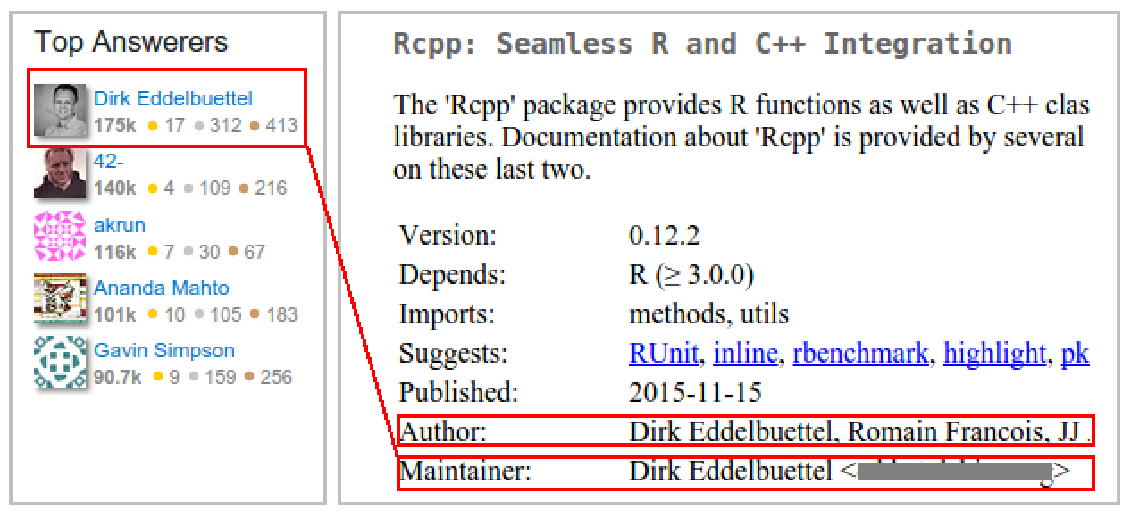
\includegraphics[width=.9\columnwidth]{Figures/CCchannel}
        \caption{Example of how to reach developers of the \emph{rcpp} package. On the left, Stack Overflow, and on the right, the \emph{rcpp} webiste.}
        \label{fig:CCchannel}
    \end{figure}

    Some channels are more suitable for certain \emph{type or format of questions}. 
    Thus, R-help mailing list is a place for discussion, and Stack Overflow is a place for questions that have a clear answer.


\subsubsection{Read the user manuals, channel rules and learn the basic concept of the technology used}

    Through the study, we noticed that most of the harsh responses from the community were give to users who did not read the posting guide or learned the basic concept for each technology (e.g., \textit{``An Introduction to R''}\footnote{\url{https://cran.r-project.org/doc/manuals/r-release/R-intro.pdf}})---users should demonstrate a minimum understanding and use of the programming language.
    The community expects that if someone wants to use a channel, they should learn about it in advance, and learn the basics of the technology that they are using.
    For instance, in the R-help's thread \textit{\href{http://goo.gl/Dc8gXw}{``Quantile''}} it is remarked the points of a guide that the user asking the question did not follow: \textit{``...Please read the Posting Guide. It asks that you not crosspost. If you post a followup to rhelp, then the reading of the Posting guide will tell you that much more in the way of detail about your setup was requested...''}.

    Depending on the channel, the amount of guide lines and posting guides available might differ. 
    Stack Overflow provides user manuals\footnote{\url{http://stackoverflow.com/help}} for each of the main features of the channel such as badges, questions, answers, flags, comments, and reputation system.
    In contrast, the R-help mailing list only has the general instructions\footnote{\url{https://www.r-project.org/mail.html\#instructions}} and the posting guide user manual\footnote{\url{https://www.r-project.org/posting-guide.html}}, which make the R-help mailing list a more user friendly environment for new users in terms of what users have to read in advance.

    Moreover, depending on the technology, there are some \textit{community} user manuals that might be useful to read before participating in the channel.
    For instance, the post on Stack Overflow \textit{``How to make a great R reproducible example?''}\footnote{\url{http://stackoverflow.com/questions/5963269/how-to-make-a-great-r-reproducible-example}} provides tips and tricks for creating a reproducible example using the R language.
    Another example is the channel related user manual written by Hadley Wickham.
    It provides some tips for posting on the R-help mailing lists: \textit{``...Before putting all of your code in an email, consider putting it on \href{http://gist.github.com/}{[GitHub Gist app]}. It will give your code nice syntax highlighting, and you don't have to worry about anything getting mangled by the email system...''}

    Finally, there are technology manuals like \textit{``An Introduction to R''}), and the FAQ webpages that are available to the public---most of the time free of charge, from which any user can learn the basic of each technology.
    For instance, the R community provides a compendium of PDF documents for new users on different languages\footnote{The R Manuals are available at \url{https://cran.r-project.org/}}.
    While on Stack Overflow, supported technologies are provisioned with webpages and links to free and paid materials\footnote{Materials available at \url{http://stackoverflow.com/tags/r/info}}.
    Members are able to reference these materials when needed, e.g., \textit{``...You may want to acquaint yourself with the 'An Introduction to R' manual that came with your R installation to learn more about indexing.''}

\subsubsection{Choose a channel according to the user experience}
            
    The variety of media channels can be overwhelming to decide in which channel post.
    It is advisable to learn the characteristics of the channels before making a decision.
    For example, using Stack Overflow has benefits such as low response time~\cite{Mamykina2011} and peer recognition~\cite{Singer2013}, but user manuals should be read prior participation.
    A bad reputation in the channel might affect users in real life~\cite{Singer2013}.
    U14 pointed that one of the biggest challenges of using Stack Overflow is learning the \emph{ethos} of the channel.
    
    Communities like R, have multiple channels with overlapping functionality.
    The R-help mailing list can be used for the same purpose as Stack Overflow, but it has a different audience, which might bring some benefits.
    For instance, the R-help mailing list is less confronting, it can be used to learn rather than just get the answer, and it can be sometimes friendlier.
    
    Squire's study~\cite{Squire2015a} as well as our findings suggest that Stack Overflow might not be enough to fully support software developers.
    As it is suggested by the amount of active users on the R-help mailing list, a community might require a place to discuss topics that are in and out of the software development domain.
    The fragmentation of topics within the Stack Exchange's Q\&A channels (each channel from Stack Exchange supports a small group of topics), the complex rules of their sites, and the gamification mechanism might be a difficult issue to handle for some users~\cite{Vasilescu2013}.

\subsubsection{Provide a background to the question}

    In spite of reading the documentation available, a user may fail to address the channel appropriately.
    The community may feel that the question asked, the information provided or something else is not in compliance with the expectations and rules of the channel.
    In such cases, one should describe the documentation read, the attempts made, and what is being trying to achieve.
    This would avoid answers like \textit{``read the manual''} or \textit{``read the posting guide''}, as well as helping the participants to help.
    As an example, in the thread \textit{\href{https://goo.gl/Gbek3R}{``lme4 GLMM''}}, a user asked \textit{``I'm very sorry for my repeated question, which I asked 2 weeks ago, namely: I'm interested in possibly simple random-part specification in the call...''}.

\subsection{Recommendations for using external resources}

    A common practice to answer or ask questions is to provide links for documentation, examples, source code, or other resources.
    As links point to online resources that might not exist in the future, it is important to include the key points of the resource within the question or answer.
    For instance, when a question or answer contains information in an external file hosting service like Dropbox or Google Drive, the owner of the service account can break the link at any moment, leaving the message incomplete or impossible to reproduce, like the thread \textit{\href{http://goo.gl/5nanFU}{``Is it possible to create a 3d contour plot without continuous data in R?''}}.
    U33 suggested: \textit{``Questions should be self-contained as much as possible. Exceptions: recognizable links such as CRAN, R documentation, etc.''}.

    Based on our observations, we constructed a set of recommendations for links that are the exception of the rule:

    \begin{description}[itemsep=3pt, topsep=2pt, leftmargin=3em, parsep=0pt]
        \item[Well known websites] are expected to be maintained in the long term like Wikipedia, the official documentation in CRAN.
        For example, the Stack Overflow's thread \textit{``calculating convolution of multinomial distribution''} a user posted \textit{`I'm doing a simulation where I need to calculate a \href{https://en.wikipedia.org/wiki/Convolution_of_probability_distributions}{[Wikipedia convolution]} of \href{https://en.wikipedia.org/wiki/Multinomial_distribution}{[Wikipedia multinomial distributions]}...''}.

        \item[Resources that support or expand the message] when the important information is already in the message.
        For instance, the Stack Overflow's thread \textit{``How do I save all the draws from a MCMC posterior distribution to a file in R''} clarifies \textit{``...You should be able to open a text connection using ?file \href{http://stat.ethz.ch/R-manual/R-devel/library/base/html/connections.html}{[more information]} with the open argument set to write...''}.

        \item[Material relevant to the message is too big] as papers or demonstrations.
        For instance, the R-help's thread \textit{``Using FUNCTION to create usable objects''} a user stated \textit{``I suspect you are trying to find your way into Circle 6 of 'The R Inferno' but haven't yet got in. \href{http://www.burns-stat.com/pages/Tutor/R\_inferno.pdf}{[R Inferno]}''}.
    \end{description}

\section{Threats to validity}
\label{cha:threats}

    In this section, we explain how we addressed each threat to
    validity.\remarks{Consider make the data available online.}

\subsection{Construct validity}

    The open coding of a large collection of messages may introduce bias.
    To minimize the bias by misinterpretation, we used multiple data sources to triangulate our findings (survey, documentation, and messages from two media channels), we randomly selected data, and two researchers performed the data coding.
    We applied the Cohen Kappa coefficient on categories that were not mutually exclusive, whose purpose  was to trigger discussion between coders.
    We set a threshold of 80\% as the minimum to obtain agreeable results, which is higher than the 60\% suggested in the literature~\cite{Landis1977}.
    We identified and reported the discrepancies and contradictions.

\subsection{Internal validity}

    To compare two different data sources, we mapped the message types between Stack Overflow and the R-help mailing.
    However, the R-help mailing list contains unstructured data, and some data may be unsuitable to compare as both data sets, R-help mailing list and Stack Overflow, have different time frames.
    To minimize unsuitable messages, we limited the analysis to the time frame that all the information was available in both data sets.
    Additionally, our understanding of that data and the observations we made played a big role in the mapping exercise, and it is subject to research bias.
    To minimized the bias, two researches performed the mapping.

\subsection{External validity}

    This study is an exploratory case study and only applies to the R community.
    A case study cannot be assumed to be generalizable until further evaluations have been conducted~\cite{Yin2009}.
    Findings in this research should be tested in other communities and with other channels to see if they apply to these other contexts.

    The R community is composed by atypical programmers.
    The R programming language is used to solve statistical problems, the final product is a script that process specific data.
    Most R language users are likely to be \textit{casual developers} with limited or non-existent programming experience, with backgrounds that vary from biologists to statisticians.
    As a consequence, this study might not represent the knowledge that a software developer community shares.

%%% Local Variables:
%%% mode: latex
%%% TeX-master: "knowledge-curation.tex"
%%% End:
